\section{Introduction}

%\subsection{Motivation}
%\label{sec:motivation}

% Importance/rise in use of GNNs

% The rise in use of ML systems

%% Wide spread of ML systems in general prevalent in every day use

\emph{Neural networks} (NN) are able to infer complex relationships within data, \emph{graph neural networks} (GNN) extend this functionality to connected systems where predetermined relationships exist between data points.
In these systems, such as social networks~\cite{pmlr-v70-gilmer17a} and molecules~\cite{DBLP:journals/corr/abs-1806-01973}, the data can be represented as nodes connected by edges in a graph.
However, the deep learning approach, of multiple layers separated by non-linear activations, has been criticised as unnecessarily complex for GNNs.~\cite{wu2019simplifying}
This is because, unlike standard NNs, the power of GNNs is hypothesised to arise from utilising the graph topology.
Thus, the ability for deep NNs to approximate arbitrary functions using non-linearity may not be required.
Instead \emph{simplified GNNs} have been proposed~\cite{chanpuriya2022simplified,chien2020adaptive,wu2019simplifying} which are either entirely linear or quasi-linear, using one or two non-linear layers.

%\begin{figure}
%    \centering
%    \captionsetup{width=0.9\textwidth}
%    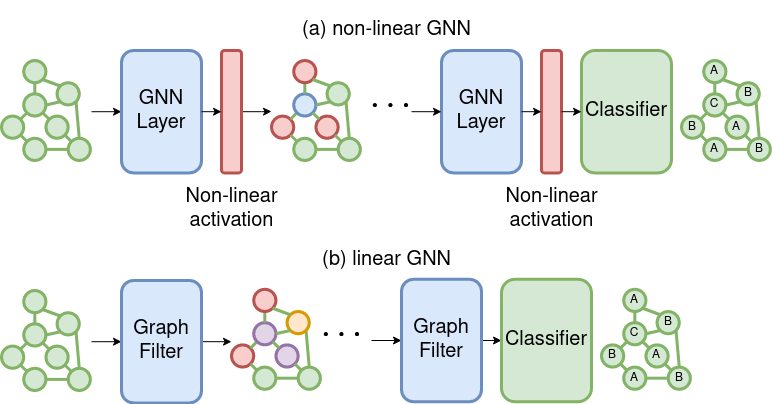
\includegraphics[width=0.8\textwidth]{figures/linear-vs-non-linear}
%    \caption{An overview of how traditional, non-linear GNNs work compared to linear GNNs. The distinction between GNN layers and graph filters is made as linearisation has focused on graph filters ignoring the more complex GNN layer approaches.}
%    \label{fig:linear-vs-non-linear}
%\end{figure}
%
%Figure \ref{fig:linear-vs-non-linear} demonstrates the difference in architecture between traditional, non-linear GNNs and linear GNNs.
These linear models have been shown to match the performance of non-linear GNNs on a limited number of datasets.~\cite{wu2019simplifying, chanpuriya2022simplified, chien2020adaptive}
However, these datasets represent a small portion of possible graph datasets and little work has been done to understand how linear GNNs work.

\begin{figure}[h]
    \centering
    \captionsetup{width=0.9\textwidth}
    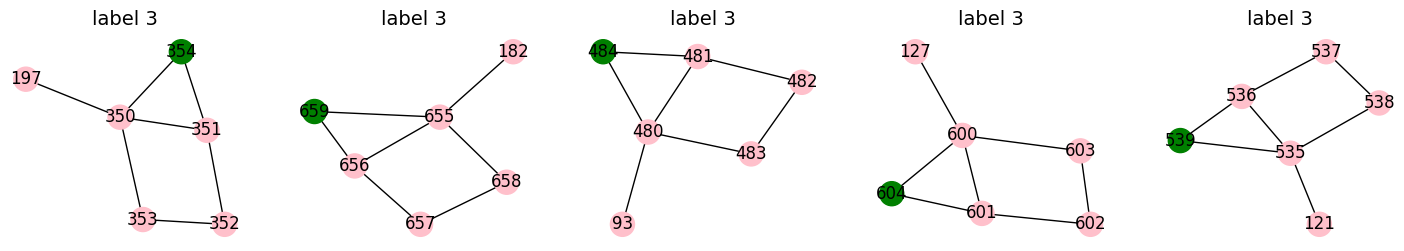
\includegraphics[width=0.95\textwidth]{figures/concept}
    \caption{An example graph concept from GCN~\cite{kipf2016semi} demonstrating that when classifying the top node the model identifies the house structure and attaching arm. The consistency of the structure suggests that this is important when classifying the top node.}
    \label{fig:concept}
\end{figure}

%\fig{concept}{An example graph concept from GCN~\cite{kipf2016semi} demonstrating that when classifying the top node the model identifies the house structure and attaching arm. The consistency of the structure suggests that this is important when classifying the top node.}

This lack of understanding extends generally to NNs where explaining how a model works is largely ignored in favour of higher accuracy.
%This approach is flawed as it is possible to create explainable architectures that do not limit accuracy~\cite{zarlenga2022concept}.
This paper combats this by analysing NNs through the subspaces in their input which influence their classification the most, these are referred to as \emph{concepts}.
This approach avoids altering the architecture and thus maintains the original accuracy achieved by the trained model.
An example of a concept is presented in Figure \ref{fig:concept} which can be interpreted as ``a house structure with an attaching arm''.
This explains how the GNN classifies the highlighted node, by identifying the house structure and attaching arm, in a human-interpretable way.

Concepts can highlight the limitations of linear GNN models, by demonstrating which graph structures and node features cannot be distinguished.
By comparing the differences in concepts between linear and non-linear models further insight into how linearity influences graph structure awareness can be gained. 
This motivates the paper which aims to provide a deeper insight into graph representational learning and provide novel techniques to graph structure inference.

%In recent years there has been rapid development and adoption of machine learning systems such as \emph{neural networks} (NN).
%However, methods to explain how these ever larger models work is lagging behind leading to either mistrust in, or worse, blind trust in these systems.
%Though standard NNs are in the mainstream spotlight there is increasing requirement for NNs to infer knowledge about connected systems such as social networks and molecules.
%The mainstream advancements result in increasingly larger \emph{neural network} (NN) models focusing on text and image based input.
%This development makes sense from the perspective of human interaction however these are limited datastructures especially in the ever increasing interaction of digital information.
%Data present in social networks, computational biology, and systems such as smart cities have multiple predefined connections between each data point.
%In these systems the connected structure is important to classification of the individual data-points leading to the concept of \emph{graph data} and the idea of the \emph{graph neural network} (GNN).
%But criticisms of the deep learning (DL) approach to GNNs has resulted in \emph{Linear GNNs} (SGNNs) that remove non-linearity and focus on the additional information provided by the graph connections.
%\note{somewhere else: How do these linear GNNs compare to non-linear GNNs in how they infer labels for graph data?}
%\note{somewhere else: Are there potential insights into how graph structure can be better utilised?}
%\note{somewhere else: This dissertation answers these questions by evaluating an SGNN within an explanability framework and provides new methods of utilising graph data in SGNNs.}

%% Brief description of evolution of GNNs, looking at motivation and use cases

%\paragraph{Graph data}
%Rather than a dataset being only a collection of feature vectors representing observed data points within the problem setting an additional adjacency matrix is also present.
%The adjacency matrix represents the connections between data points that is inherently present in the observed data.
%An example being friendship connections in a social network or bonds between atoms in a molecule.
%This additional structure provides useful information for tasks where the interaction between data points has importance to the data points themselves.
%More complex graph data may also include attributes associated with the connections which can be simple scalars or multidimensional vectors.
%For these reasons graph data is a highly flexible and versatile datastructure promoting complex inference.

%\paragraph{Graph neural networks (GNNs)} 
%are designed to handle graph data where the connections between data points is an important aspect as the data itself.
%The standard form of a GNN 
%\note{make sure this is valid here!}
%consists of multiple layers connected together by a non-linearity step.
%Each layer performs inference on a node's feature vector in the same way as a NN would perform inference.
%The graph structure is utilised by broadcasting this new node representation along the connected edges to neighbouring nodes.
%Each node then aggregates the representations of its neighbouring nodes creating a compact representation of the neighbourhood according to itself.
%The updated representation and aggregation are then combined to produce a final representation before the next layer.
%By using a process known as \emph{message passing} each node's feature vector is updated based on the graph neighbourhood inferring graph structure as well.
%This process, known as \emph{message passing}, allows a GNN to utilise the graph structure and infer more complex relationships between the data points than an ordinary NN.

%% Rapid integration of these systems 

% The lack of clarity in ML systems
% -> Explainability
% -> Concepts

%\paragraph{Linearising NNs}
%Modern specialist computer hardware, such as graphics processing units (GPU), are incredibly efficient at carrying out large linear operations such as matrix multiplication.
%However, the vast majority of NNs contain non-linear operators between generally linear layers.
%The idea of linearising NNs is to remove \emph{some} of the non-linearity in the architecture multiple layers to be combined into a single linear operation.
%Removal the early non-linearity (or all the non-linearity) results in a pre-computation step that can be carried out on an entire dataset before training or inference.
%%Thus in cases where inputs are sampled from a collection of data points this prevents calculating the same operation on the same data point across samples.
%But, it is important that this does not effect the performance of the model.

%\paragraph{Linear GNNs}
%The process of message passing though complex conceptually can easily be decomposed into a linear operation on the graph features and graph adjacency.
%Using the idea of linearising NNs the non-linearity between individual message passing layers can be removed.
%This allows a GNN to pre-compute multiple message passing steps on the graph dataset before inference.
%Inference then results in a simple classification or linear regression task where only a single layer is required.
%This new \emph{linear GNN} (SGNN) remove their non-linear complexities whilst demonstrating comparable performance to standard GNNs.

%\paragraph{Explainability}
%The advancement of new NNs has focused on improving the performance in metrics such as accuracy and training cost which has resulted in impressive models.
%However, these models remain as blackboxes to the users of these systems but equally to the designers.
%Once a model is trained on a specific dataset there is very limited understanding of how the model is analysing the input to produce a result.
%This can and does create a lot of mistrust in NNs as there is a large element of trusting that the output it produces on unseen data will match our expectation.
%The idea of explainability is to provide different methods of visualising how a model works to a human as a form of verification or to provide insight.
%Many different approaches exist including before, during and after training, to varying degrees of explanation.

%% Importance of understanding ML inference
%% -> Link to potential use cases 

%% Issues with interfering with training

%% Recent development in developing frameworks to analyse these aspects
%% The different goals of explainability 

%\paragraph{Concepts}
%A specific form of explainability that is applied after the training of a model \note{Check that this is always the case!} is that of concepts.
%The idea is to find different subspaces of the input space (where each input to tthe NN is some element of the input space) that correspondent to a specific output.
%This way patterns can be found between input and output to verify that the model is behaving as expected.
%In this dissertation the focus is on graph concepts which are subgraphs created from the input graph(s) for the model.
%These subgraphs represent the graph structures that the model is using to carry out inference on specific inputs.
%
%\paragraph{Concepts in simplified GNNs}
%Though SGNNs show competitive performance when looking at classification accuracy they are a black box as with the majority of NNs.
%As SGNNs delay the influence of the models weights until the final classification step this provides an opportunity to see how graph concepts are effected.
%If these models are truly comparable to GNNs then the concepts should demonstrate how the message passing steps operate.
%These results could therefore influence the design of future networks as the DL approach may not be required for graph data. \note{This needs better wording, I don't know how much I agree with it myself.}

%% The idea of a concept
%% The fact in our case this is done after training
%% -> This does not effect training performance

% More efficient systems should not sacrifice ease of understanding

%This project applies the graph explainability tools proposed by \citet{magister2021gcexplainer} to the linear model SGC~\cite{wu2019simplifying}.
This paper provides a new analysis of linear GNN models and their limitations providing new insight into how graph structure is inferred.
These results demonstrate that purely linear models, such as SGC, cannot infer fine-grained graph structure and are instead optimised for tabular data.
We hypothesise that this limitation is due to limited access to intermediate node representations during classification.

In this work we make the following contributions:
\begin{itemize}
    \item 
        We demonstrate that the current approaches to linearising GNNs are limited by their inability to infer graph structure.
    \item 
        We introduce SGCN, a quasi-linear model that exploits the efficient SGC pre-computation but retains some GCN layers to maintain high accuracy.
    \item
        We introduce JSGC, a quasi-linear model that provides the classification layer with intermediate node representations to demonstrate that this is a major bottleneck in linear models.
\end{itemize}

